\section{Τεχνητά Νευρωνικά Δίκτυα}
Τα τεχνητά νευρωνικά δίκτυα (\emph{Artificial Neural Networks - ANN}) αποτελούν υπολογιστικά συστήματα τα οποία είναι εμπνευσμένα από τα βιολογικά νευρωνικά δίκτυα που συναντώνται στη φύση (π.χ στον ανθρώπινο εγκέφαλο). Τα \emph{ANN} αποτελούνται από κόμβους, σε αντιστοιχία με τους νευρώνες, που μπορούν να είναι συνδεδεμένοι με άλλους κόμβους, σε αντιστοιχία με τις συνάψεις του εγκεφάλου.

Η πιο απλή δομή ενός νευρωνικού δικτύου είναι ο νευρώνας (\emph{perceptron}) και μπορεί να παρουσιαστεί με το \autoref{fig:perceptron}. Οι είσοδοι στο νευρώνα πολλαπλασιάζονται με ένα βάρος η κάθε μία και στη συνέχεια αθροίζονται, παράγοντας έτσι το ζυγισμένο άθροισμα των εισόδων. Το αποτέλεσμα του νευρώνα υπολογίζεται με το πέρασμα του αθροίσματος από μία συνάρτηση ενεργοποίησης. Στην απλούστερη περίπτωση η συνάρτηση ενεργοποίησης μπορεί να παραληφθεί και το αποτέλεσμα του αθροίσματος να είναι η έξοδος του συστήματος. Σε περίπτωση που υπάρχει, είναι αυτή που καθορίζει την έξοδο του νευρώνα (αν θα ενεργοποιηθεί ο νευρώνας ή όχι). Υπάρχουν διάφοροι τύποι συναρτήσεων ενεργοποίησης που χρησιμοποιούνται για τεχνητά νευρωνικά δίκτυα με τις κυριότερες\footnote{\url{https://en.wikipedia.org/wiki/Activation_function}}:

\begin{itemize}
    \item \textbf{δυαδική (\emph{binary})} - η έξοδος είναι \{0, 1\}
    \item \textbf{σιγμοειδής (\emph{sigmoid})} - η έξοδος είναι στο [0 1]
    \item \textbf{υπερβολική εφαπτομένη (\emph{tanh})} - η έξοδος είναι στο [-1 1]
    \item \textbf{Rectified Linear Unit - ReLU} -  η οποία θέτει την έξοδο ίση με το μηδέν σε περίπτωση αρνητικών τιμών, διαφορετικά δεν επιδρά στην είσοδο
\end{itemize}

\begin{figure}[!ht]
  \centering
  \captionsetup{justification=centering}
  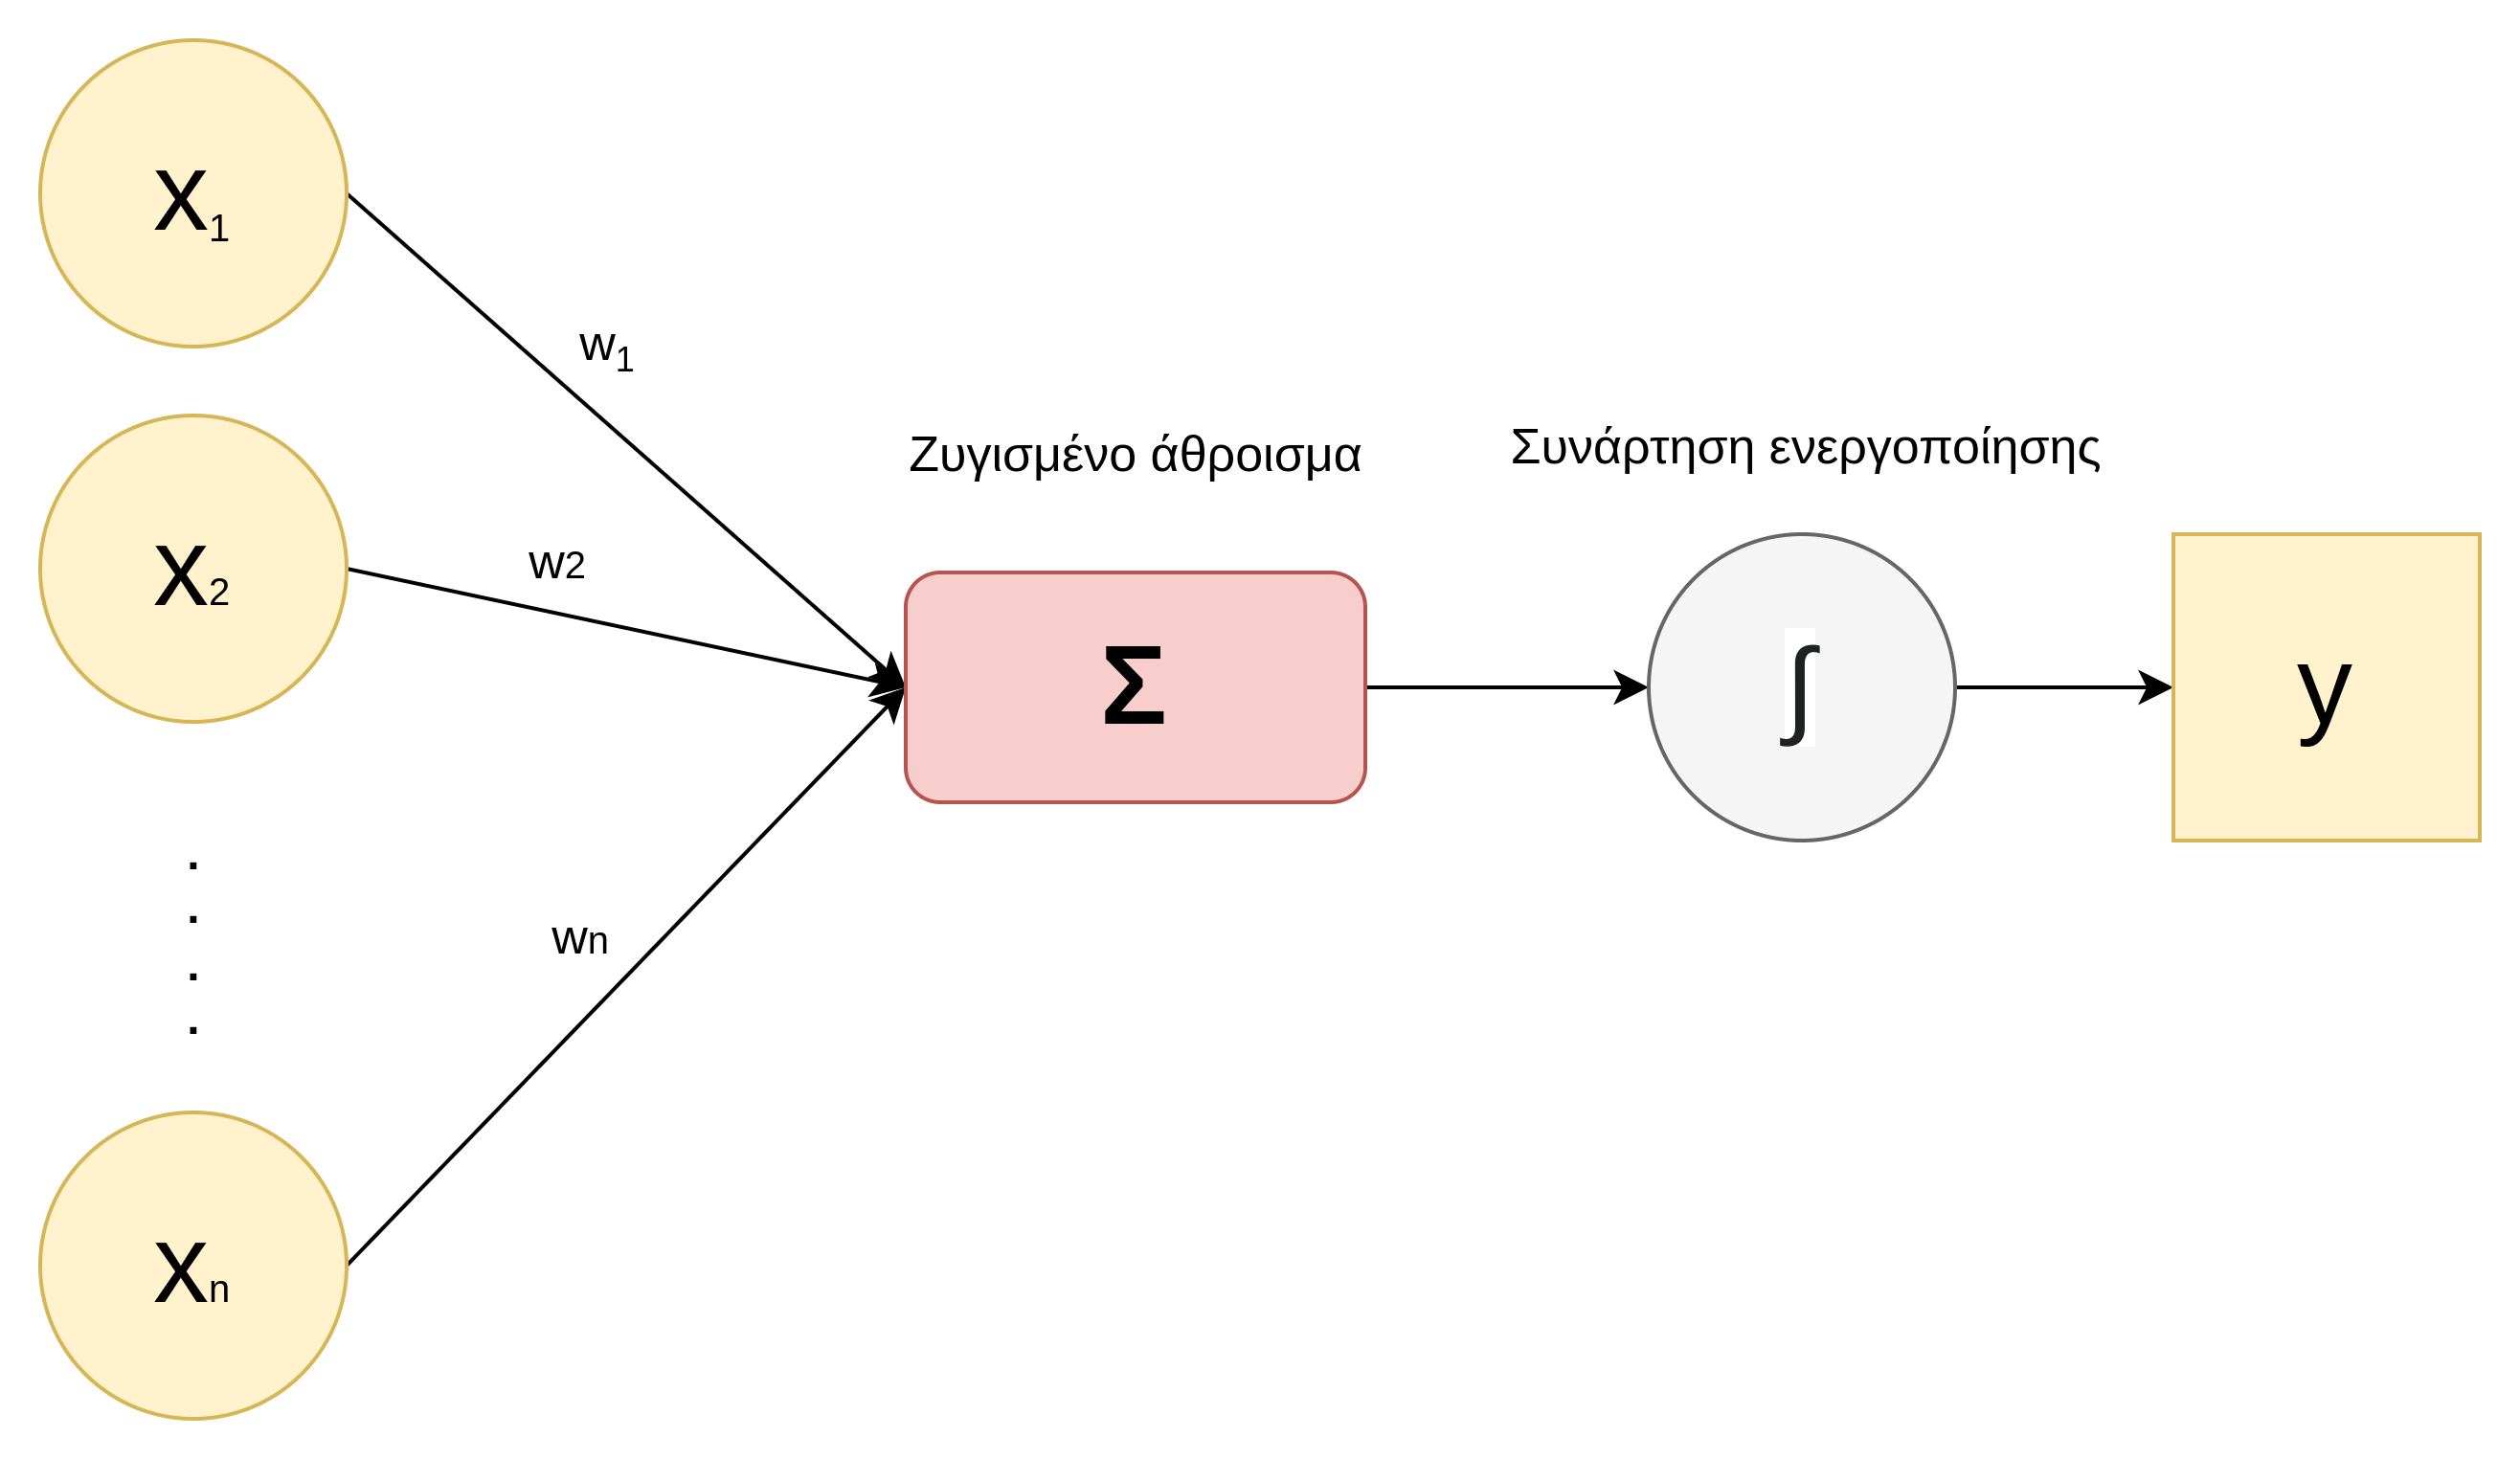
\includegraphics[width=0.7\textwidth]{images/chapter2/perceptron.png}
  \caption{\emph{Νευρώνας - Perceptron}}
  \label{fig:perceptron}
\end{figure}
\noindent

Η σύνδεση πολλών νευρώνων μεταξύ τους δημιουργεί ένα νευρωνικό δίκτυο. Νευρώνες με κοινές εισόδους σχηματίζουν μία ομάδα που ονομάζεται επίπεδο (\emph{layer}). Ένα \emph{NN} μπορεί να αποτελείται από πολλά \emph{layers}. Κάθε επίπεδο που βρίσκεται ανάμεσα στα επίπεδα εισόδου και εξόδου ονομάζεται κρυφό (\emph{hidden layer}). 
Τα \emph{NN} μπορούν να χωριστούν σε δύο κατηγορίες ανάλογα με τη ροή πληροφορίας τους:
\begin{itemize}
    \item \textbf{προς τα εμπρός (\emph{feed forward NN})} - δεν σχηματίζονται κύκλοι ανάμεσα στους κόμβους
    \item \textbf{αναδρομικά (\emph{recurrent NN})} - σχηματίζονται κύκλοι ανάμεσα στους κόμβους
\end{itemize}

Η βασική δομή ενός \emph{NN} φαίνεται στο \autoref{fig:mlp}. Αν κάθε κόμβος από κάθε επίπεδο συνδέεται με κάθε κόμβο του επόμενου επιπέδου τότε το νευρωνικό δίκτυο ονομάζεται πλήρως συνδεδεμένο (\emph{fully connected}). Επίσης, ένα \emph{feed forward NN} ονομάζεται και \emph{Multi-Layer Perceptron - MLP}.

\begin{figure}[!ht]
  \centering
  \captionsetup{justification=centering}
  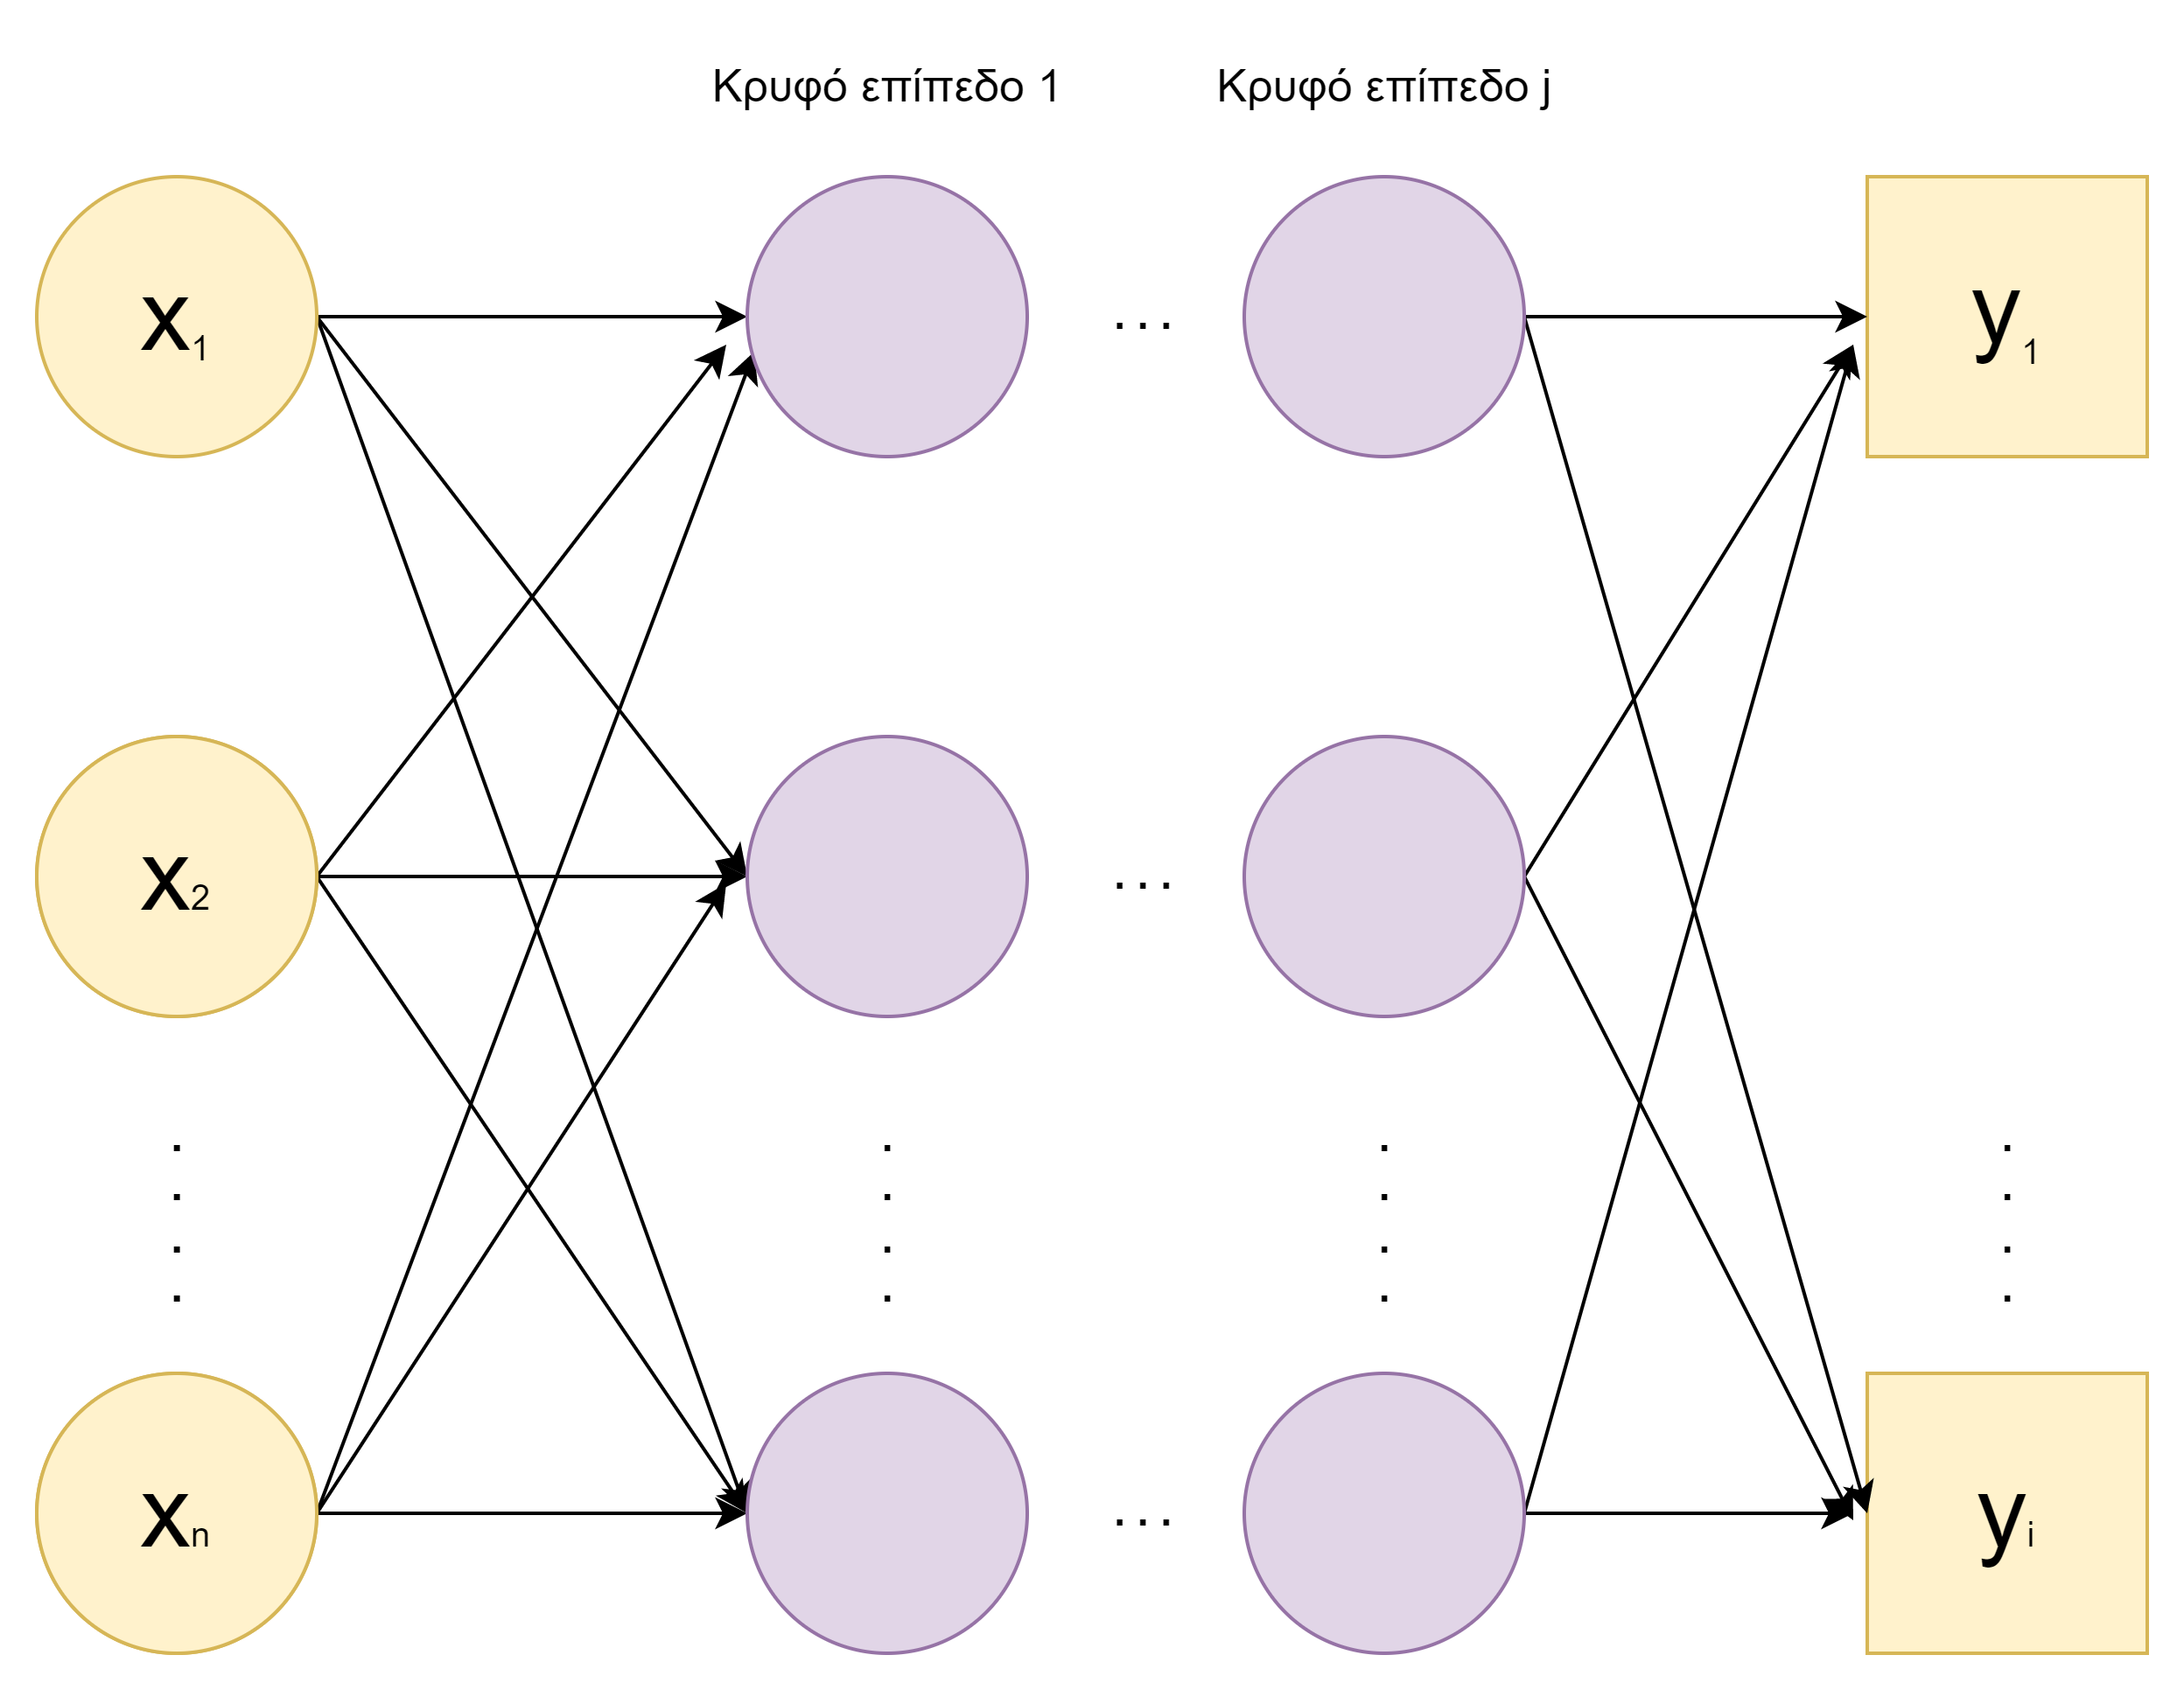
\includegraphics[width=0.7\textwidth]{images/chapter2/mlp.png}
  \caption{\emph{Feed forward Neural Network / Multi Layer Perceptron}}
  \label{fig:mlp}
\end{figure}
\noindent

\section{Ταξινόμηση με \emph{MLP}}
Συχνά μοντέλα \emph{MLP} χρησιμοποιούνται για ταξινόμηση της εισόδου σε κάποια κατηγορία (κλάση). Αν οι διαθέσιμες κλάσεις ταξινόμησης είναι δύο, τότε η έξοδος του \emph{NN} είναι μία και μπορεί να παίρνει τις τιμές $0$ ή $1$, επομένως στο τέλος χρησιμοποιείται μία \emph{sigmoid} συνάρτηση ενεργοποίησης. Σε περίπτωση που οι κλάσεις είναι περισσότερες, τότε οι έξοδοι του έχει νόημα να εκφράζουν μία συνάρτηση μάζας πιθανότητας. Πιο συγκεκριμένα, κάθε μία από τις εξόδους εκφράζει την πιθανότητα η είσοδος να ανήκει σε μία από τις κλάσεις. Το συνολικό άθροισμα των πιθανοτήτων αυτών είναι μονάδα. Η έξοδος με τη μεγαλύτερη πιθανότητα καθορίζει και την κλάση ταξινόμησης της εισόδου. Αυτό επιτυγχάνεται με τη συνάρτηση \emph{softmax} η οποία φαίνεται στην \autoref{eq:softmax}.

\begin{equation}
    \label{eq:softmax}
    \text{y}(x_{i}) = \text{softmax}(x_{i}) = \frac{\exp(x_i)}{\sum_1^j \exp(x_j)}
\end{equation}

\section{Αναδρομικά Νευρωνικά Δίκτυα}
Τα απλά \emph{feed forward} νευρωνικά δίκτυα παράγουν την έξοδο τους βασιζόμενα μόνο στα δεδομένα της τρέχουσας εισόδου. Ωστόσο, πολλές φορές η πληροφορία που παρέχεται από τα προηγούμενα δείγματα της εισόδου ενδέχεται να επηρεάζει το αποτέλεσμα της επόμενης εξόδου. Το πρόβλημα αυτό έρχονται να λύσουν τα Αναδρομικά Νευρωνικά Δίκτυα (\emph{Recurrent Neural Networks - RNN}). Ένα \emph{RNN}, \autoref{fig:rnn}, μπορεί να θεωρηθεί ως πολλά αντίγραφα ενός απλού νευρωνικού δικτύου με το κάθε ένα να παρέχει την έξοδο του στο επόμενο. Η έξοδος αυτή ονομάζεται κρυφή κατάσταση (\emph{hidden state}) και είναι αυτή που παρέχει τη "μνήμη" στο συνολικό σύστημα. Αυτή η αλυσιδωτή δομή επιτρέπει την πρόβλεψη σειριακών δεδομένων όπως χρονοσειρές, ήχο, βίντεο, δεδομένα καιρού, κείμενο και άλλων.

\begin{figure}[!ht]
  \centering
  \captionsetup{justification=centering}
  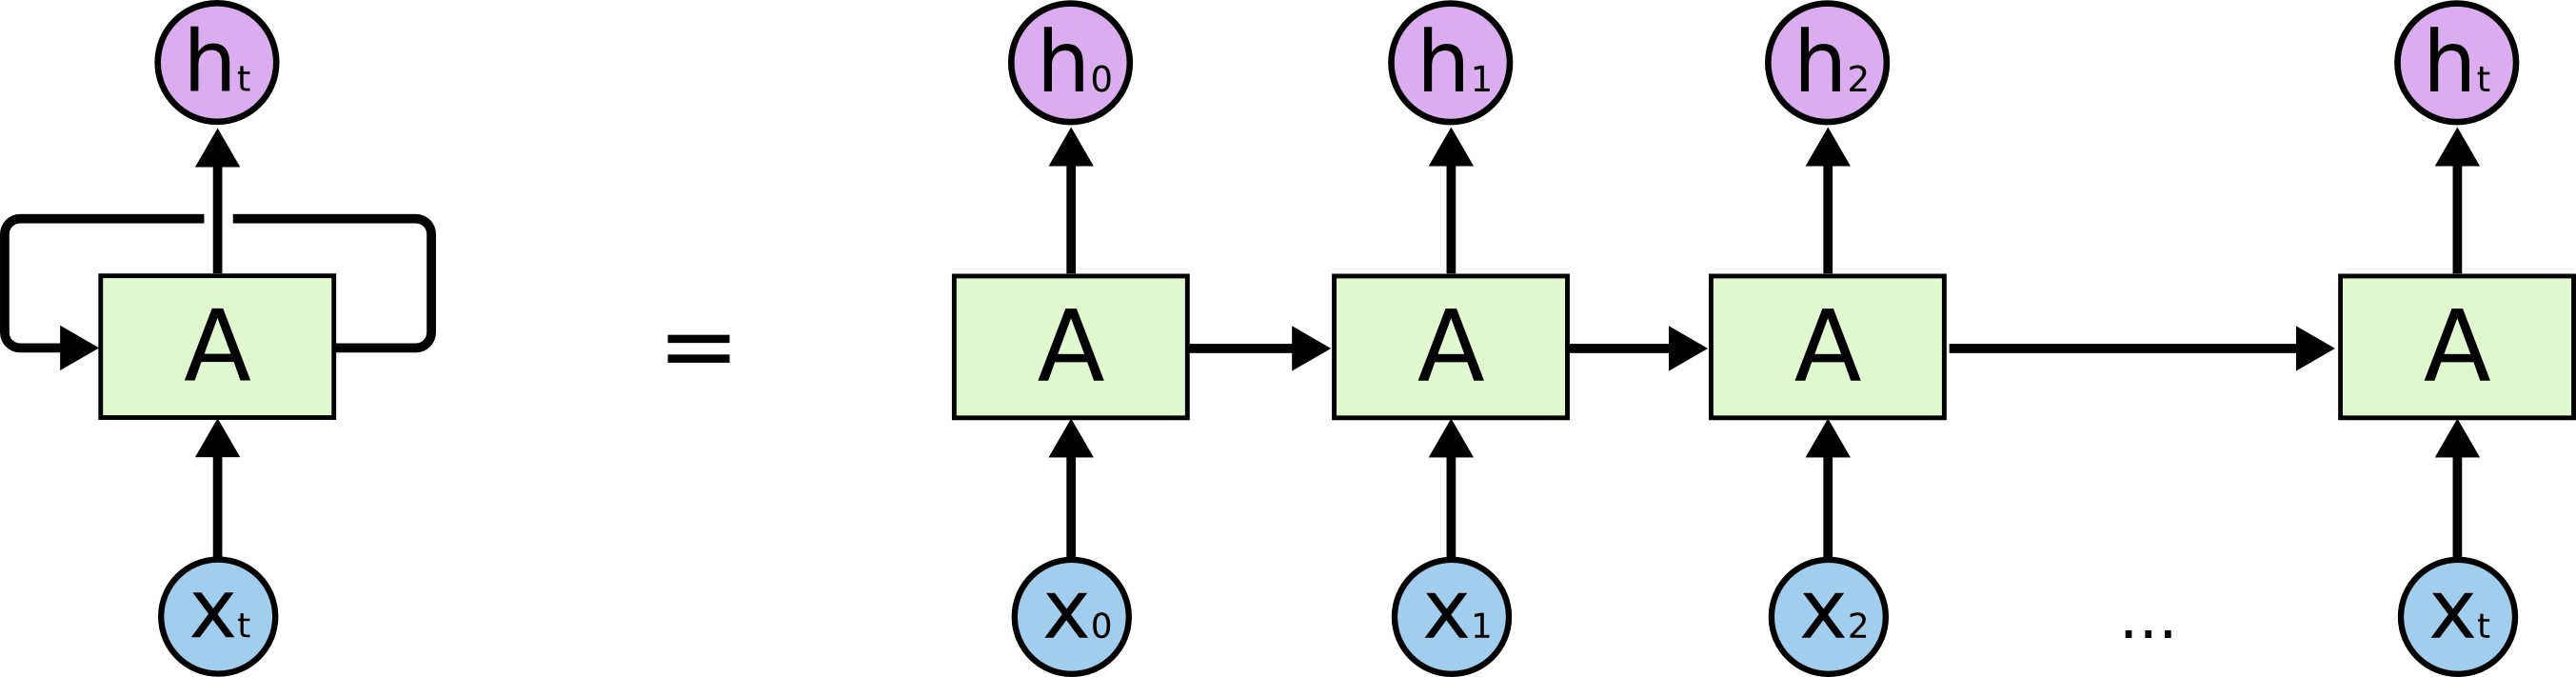
\includegraphics[width=0.7\textwidth]{images/chapter2/rnn.png}
  \captionsource{\emph{Recurrent Neural Network}}{\url{https://colah.github.io/posts/2015-08-Understanding-LSTMs}}
  \label{fig:rnn}
\end{figure}
\noindent

\subsection{Νευρωνικά Δίκτυα Μακροπρόθεσμης Μνήμης}
Παρά το γεγονός ότι τα \emph{RNN} στη θεωρία μπορούν να διαχειρίζονται συνδέσεις των δεδομένων διάφορων εισόδων, όσο εισέρχονται νέα δείγματα στο σύστημα τόσο δυσκολότερη είναι η σύνδεση με τα πιο παλιά. Αυτό το πρόβλημα είναι γνωστό στη βιβλιογραφία ως \emph{vanishing gradient descent}. Μία νέα αρχιτεκτονική, τα μοντέλα μακροπρόθεσμης μνήμης (\emph{Long-Short Term Memory - LSTM}), η οποία παρουσιάζεται στο \autoref{fig:lstm-arch}, λύνει το συγκεκριμένο πρόβλημα. Το βασικότερο στοιχείο ενός \emph{LSTM} είναι η κατάσταση του (\emph{cell state - C}), στο οποίο διατηρείται η πληροφορία από τα προηγούμενα επίπεδα. Σε κάθε επόμενο επίπεδο παρέχεται η πληροφορία του \emph{cell state} του προηγούμενου επιπέδου και υπάρχει η δυνατότητα προσθήκης και αφαίρεσης πληροφορίας σε αυτό.

\begin{figure}[!ht]
  \centering
  \captionsetup{justification=centering}
  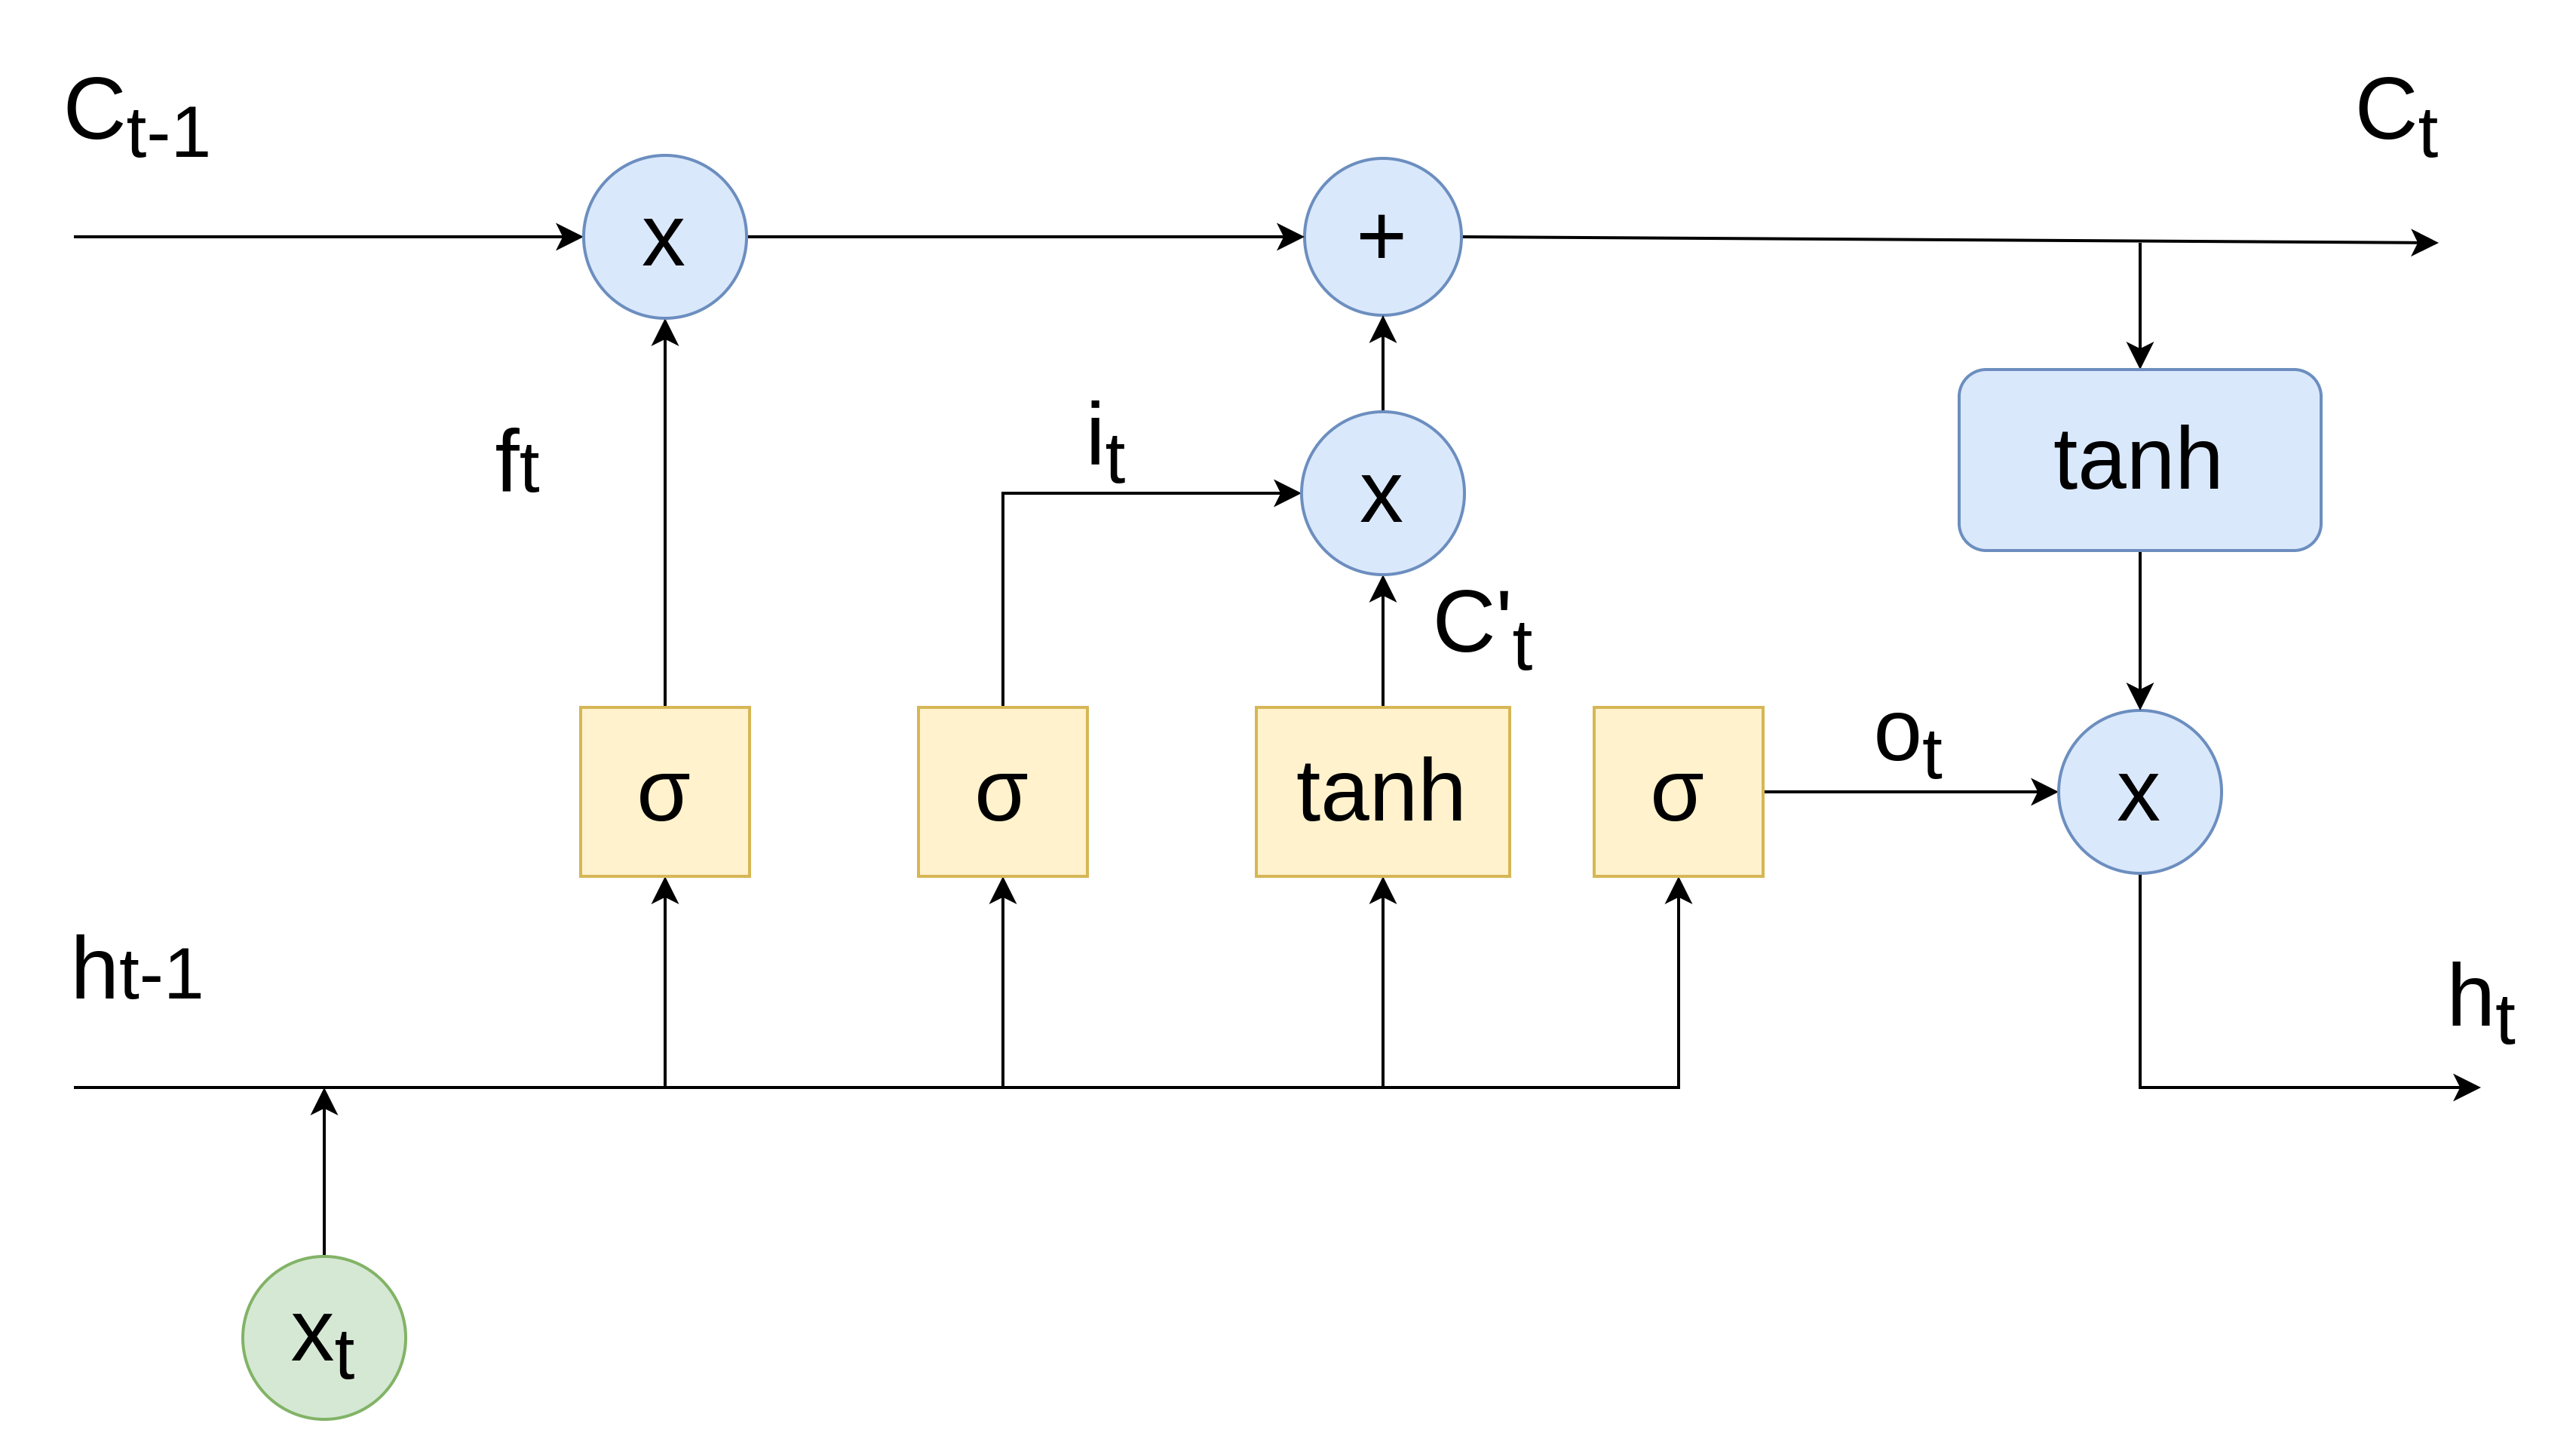
\includegraphics[width=0.7\textwidth]{images/chapter2/lstm-arch.png}
  \captionsource{\emph{Αρχιτεκτονική LSTM}}{\url{https://colah.github.io/posts/2015-08-Understanding-LSTMs}}
  \label{fig:lstm-arch}
\end{figure}
\noindent

Ο τρόπος με τον οποίο γίνεται η ανανέωση της πληροφορίας περιγράφεται στη συνέχεια. Κάθε ένα από τα στάδια επεξεργασίας μπορεί να παρομοιαστεί με το πέρασμα από μία πύλη. Στο πρώτο βήμα, πραγματοποιείται η απόφαση για το ποια πληροφορία από το προηγούμενο \emph{cell state} θα παραληφθεί, πύλη \emph{forget}. Πιο συγκεκριμένα, χρησιμοποιεί πληροφορία από το προηγούμενο επίπεδο σε συνδυασμό με την είσοδο. Η πληροφορία περνάει από μία σιγμοειδή συνάρτηση ενεργοποίησης που έχει ως έξοδο ένα διάνυσμα αριθμών, με τόσες θέσεις όσες και το $C_{t-1}$, στο διάστημα [0 1] όπου το 0 μεταφράζεται σε απόρριψη του συγκεκριμένου κελιού και το ένα σε διατήρηση του. Στη συνέχεια, γίνεται ο υπολογισμός δύο διανυσμάτων, ενός για ανανέωση ήδη υπάρχουσας πληροφορίας ($i_t$ ,χρησιμοποιώντας ξανά σιγμοειδή συνάρτηση ενεργοποίησης) και ενός για προσθήκη νέας ($C_t'$, χρησιμοποιώντας \emph{tanh} συνάρτηση ενεργοποίησης), πύλη ανανέωσης/προσθήκης. Από τον συνδυασμό των δύο διανυσμάτων αυτών προκύπτει η νέα κατάσταση \emph{C}. Η συνολική κατάσταση του επιπέδου μπορεί να περιγραφεί με τις παρακάτω εξισώσεις\footnote{Το σύμβολο $\circ$ υποδηλώνει πολλαπλασιασμό στοιχείο προς στοιχείο}:
\begin{itemize}
    \item $f_t$ = $\sigma(W_f x_t + U_f h_{t-1} + b_f)$
    \item $i_t$ = $\sigma(W_i x_t + U_i h_{t-1} + b_i)$
    \item $o_t$ = $\sigma(W_o x_t + U_o h_{t-1} + b_o)$
    \item $C_t'$ = $\sigma(W_c x_t + U_c h_{t-1} + b_c)$
    \item $C_t$ = $f_t \circ c_{t-1} + i_t \circ C_t'$
    \item $h_t$ = $o_t \circ \sigma(C_t)$
\end{itemize}

όπου: 
\begin{itemize}
    \item $x_t$: είσοδος του \emph{LSTM}
    \item $f_t$: διάνυσμα που προκύπτει από την πύλη \emph{forget}
    \item $i_t$: διάνυσμα που προκύπτει από την πύλη ανανέωσης/προσθήκης
    \item $o_t$: διάνυσμα που προκύπτει από την πύλη εξόδου
    \item $h_t$: διάνυσμα κρυφής κατάστασης του \emph{LSTM}
    \item $C_t'$: διάνυσμα για τη προσθήκη νέας πληροφορίας
    \item $C_t$: διάνυσμα κατάστασης του \emph{LSTM}
    \item W, U: πίνακες με τα βάρη που προκύπτουν από την εκπαίδευση του μοντέλου
    \item $b_f$ : είναι ένα \emph{bias} διάνυσμα που προκύπτει από την εκπαίδευση του μοντέλου
\end{itemize}